% =====================================================================
%  Universitas Pandrosion --- combined edition
%  Master document that assembles the nine papers (0..8) into a single
%  PDF via pdfpages. Each chapter includes the already-compiled PDF of
%  the corresponding paper, so every internal cross-reference, label,
%  bibliography entry, and hyperlink of each paper is preserved
%  verbatim (no renumbering, no clash between duplicate labels).
%
%  Build:
%      tectonic universitas_pandrosion_combined.tex
%  (requires the nine *.pdf files to be present in the same directory)
% =====================================================================

\documentclass[11pt,a4paper]{book}

\usepackage[utf8]{inputenc}
\usepackage[T1]{fontenc}
\usepackage{lmodern}
\usepackage[english]{babel}
\usepackage{pdfpages}
\usepackage{hyperref}
\usepackage{bookmark}

\hypersetup{
  pdftitle={Universitas Pandrosion --- Combined Edition},
  pdfauthor={Ivan Besevic},
  pdfsubject={Pandrosion-Steffensen iteration and companion papers on Smale's MVC},
  colorlinks=true,
  linkcolor=blue,
  urlcolor=blue,
  citecolor=blue,
  bookmarksnumbered=true,
  bookmarksopen=true
}

\title{Universitas Pandrosion \\ \Large Combined Edition (Papers 0--8)}
\author{Ivan Besevic}
\date{April 2026}

\begin{document}

\frontmatter
\maketitle

\tableofcontents

\mainmatter

% ------------------------------------------------------------------
% Paper 0 --- Pandrosion-Steffensen for z^p = x (Lean-verified)
% ------------------------------------------------------------------
\bookmarksetup{startatroot}
\addtocontents{toc}{\protect\vspace{0.5em}}
\chapter*{Paper 0 --- Pandrosion-Steffensen for \texorpdfstring{$z^p = x$}{z\^{}p = x} (Lean-verified)}
\addcontentsline{toc}{chapter}{Paper 0 --- Pandrosion-Steffensen for $z^p = x$ (Lean-verified)}
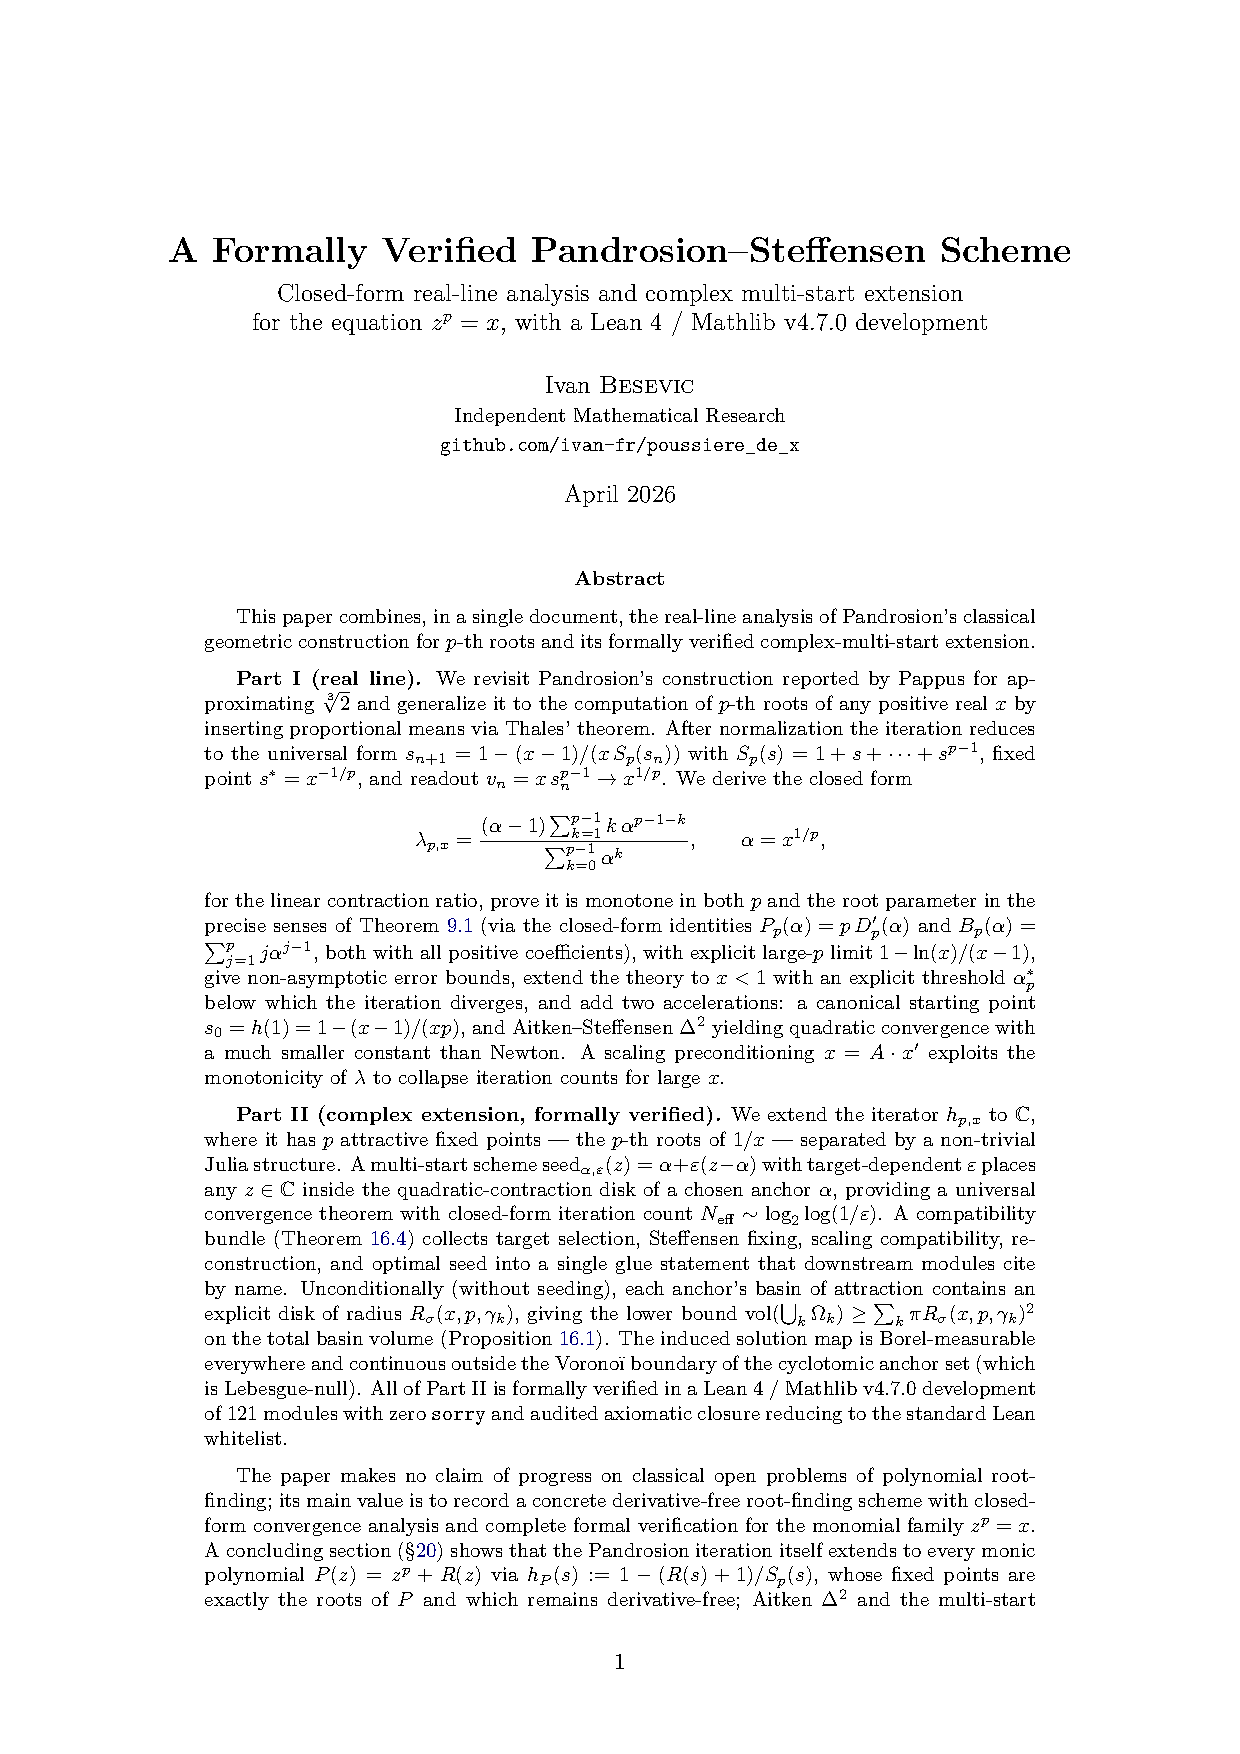
\includepdf[pages=-,pagecommand={},fitpaper=true]{0pandrosion_pth.pdf}

% ------------------------------------------------------------------
% Part I --- Univariate and multivariate adaptive-anchor Pandrosion
% ------------------------------------------------------------------
\bookmarksetup{startatroot}
\chapter*{Part I --- Adaptive-anchor Pandrosion, univariate and multivariate}
\addcontentsline{toc}{chapter}{Part I --- Adaptive-anchor Pandrosion, univariate and multivariate}
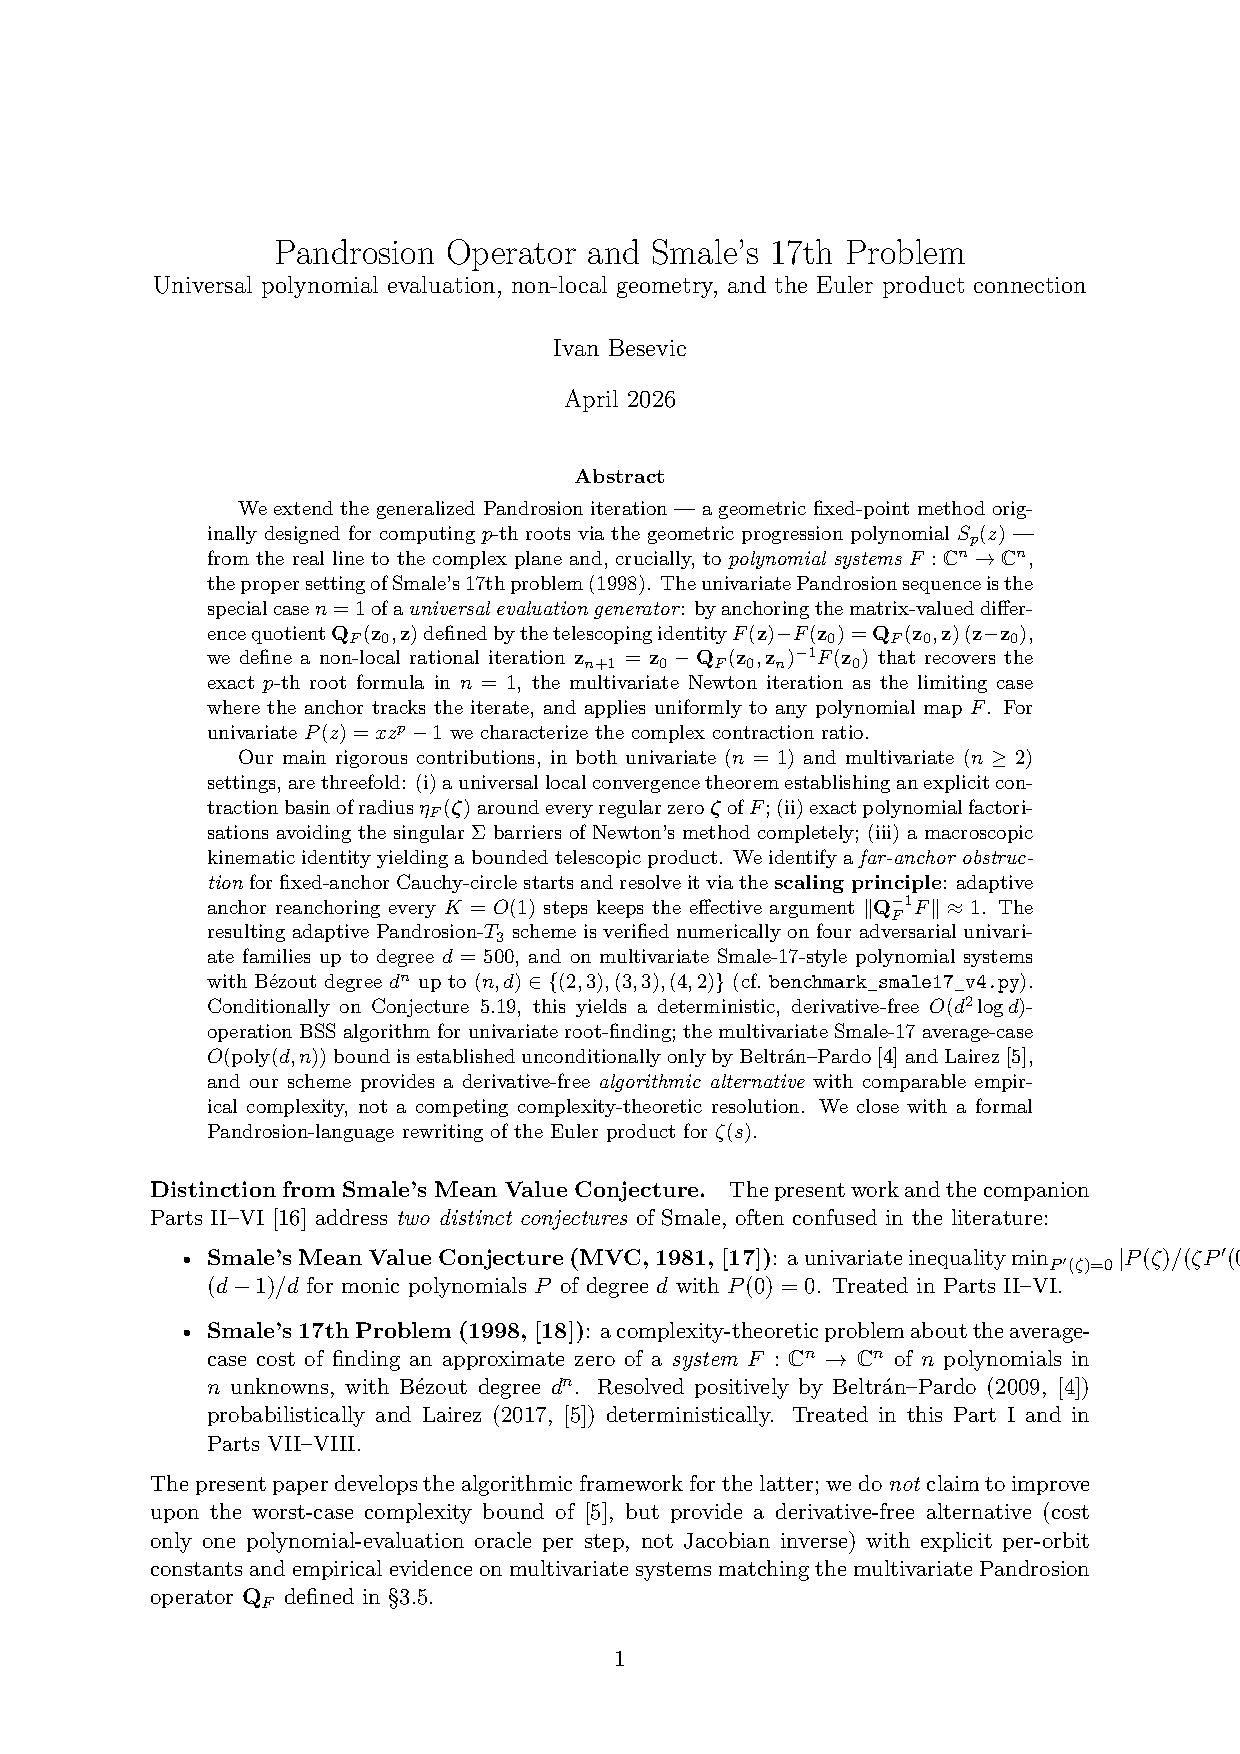
\includepdf[pages=-,pagecommand={},fitpaper=true]{1pandrosion_smale.pdf}

% ------------------------------------------------------------------
% Part II --- Smale's Mean Value Conjecture as a Pandrosion ratio bound
% ------------------------------------------------------------------
\bookmarksetup{startatroot}
\chapter*{Part II --- Smale's Mean Value Conjecture as a Pandrosion ratio bound}
\addcontentsline{toc}{chapter}{Part II --- Smale's Mean Value Conjecture as a Pandrosion ratio bound}
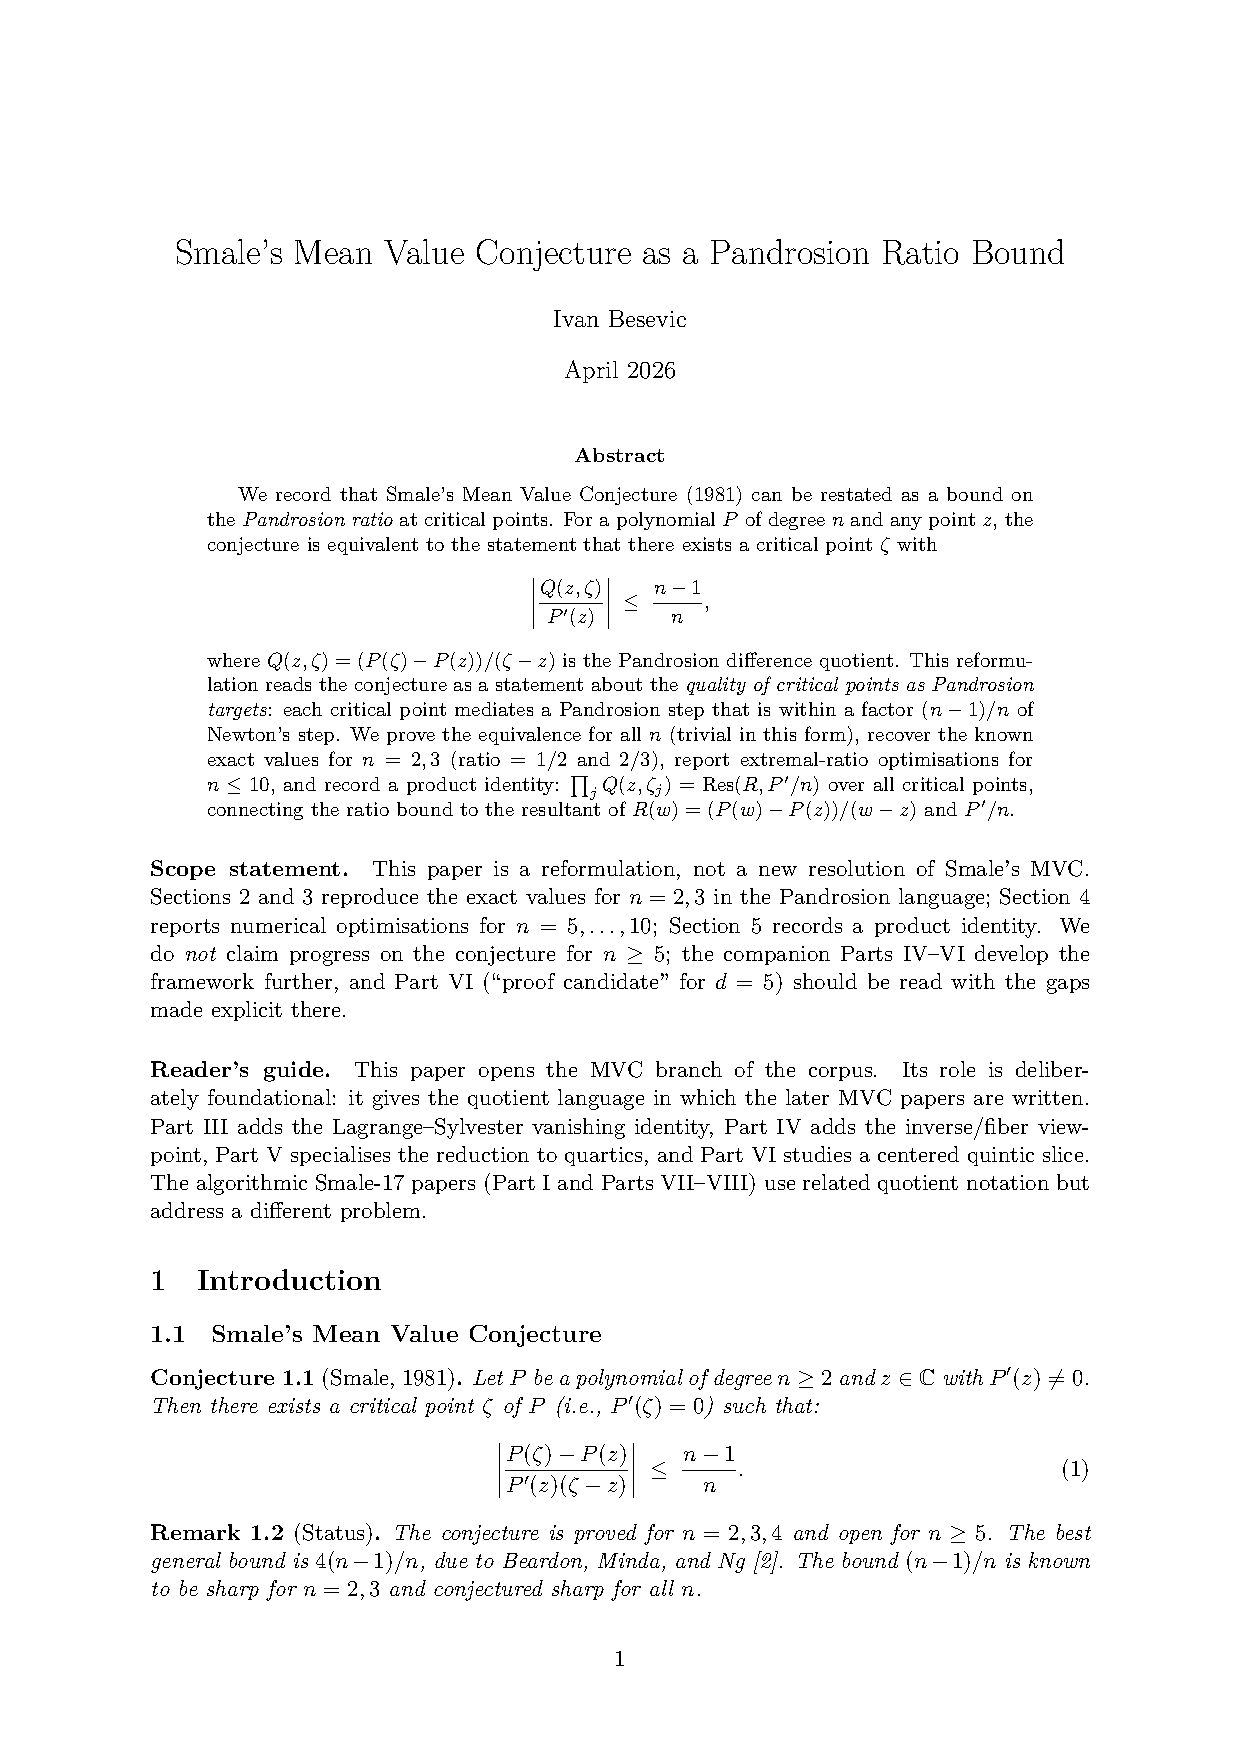
\includepdf[pages=-,pagecommand={},fitpaper=true]{2pandrosion_smale.pdf}

% ------------------------------------------------------------------
% Part III --- Lagrange-Sylvester vanishing identity
% ------------------------------------------------------------------
\bookmarksetup{startatroot}
\chapter*{Part III --- Lagrange--Sylvester vanishing identity}
\addcontentsline{toc}{chapter}{Part III --- Lagrange--Sylvester vanishing identity}
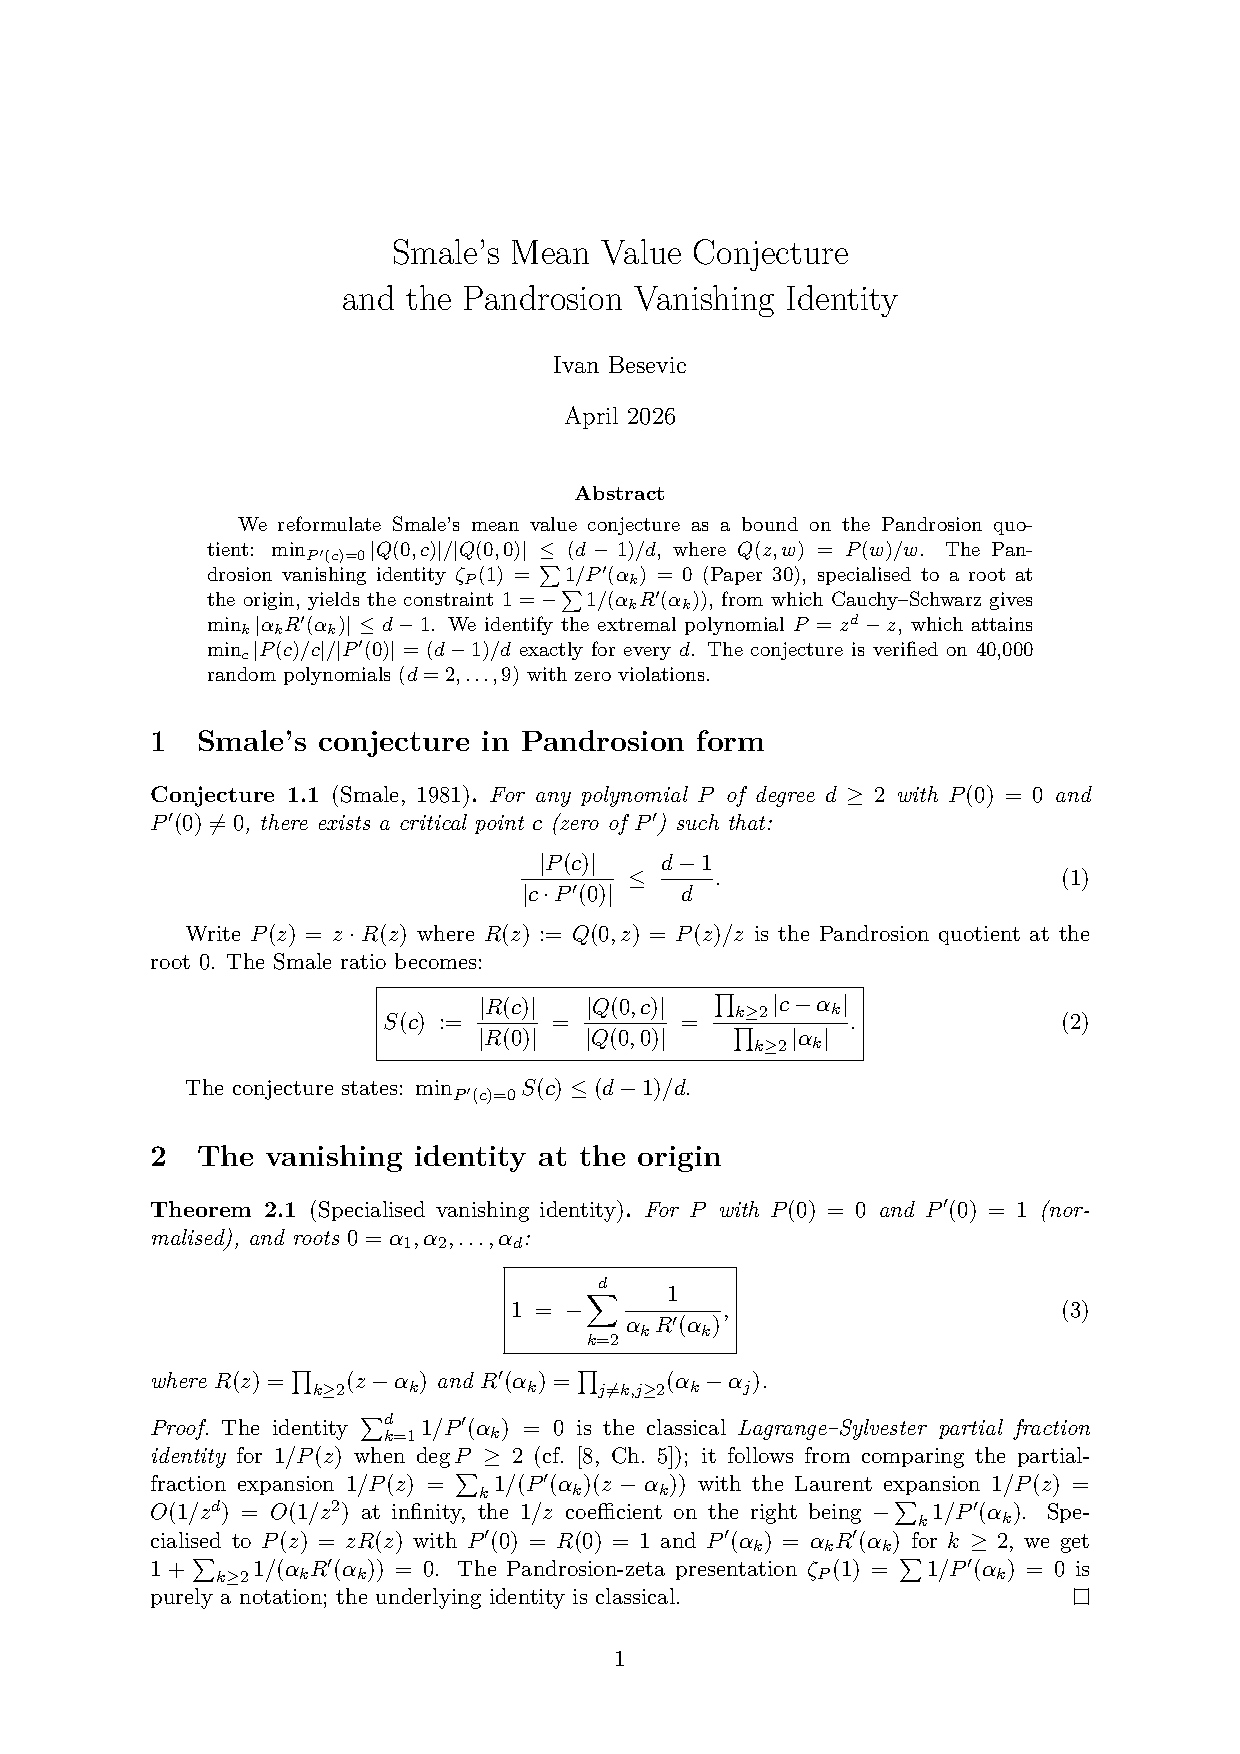
\includepdf[pages=-,pagecommand={},fitpaper=true]{3pandrosion_smale.pdf}

% ------------------------------------------------------------------
% Part IV --- Pandrosion inverse, fiber identity, Smale MVC for d=3
% ------------------------------------------------------------------
\bookmarksetup{startatroot}
\chapter*{Part IV --- Pandrosion inverse, fiber identity, Smale MVC for \texorpdfstring{$d=3$}{d=3}}
\addcontentsline{toc}{chapter}{Part IV --- Pandrosion inverse, fiber identity, Smale MVC for $d=3$}
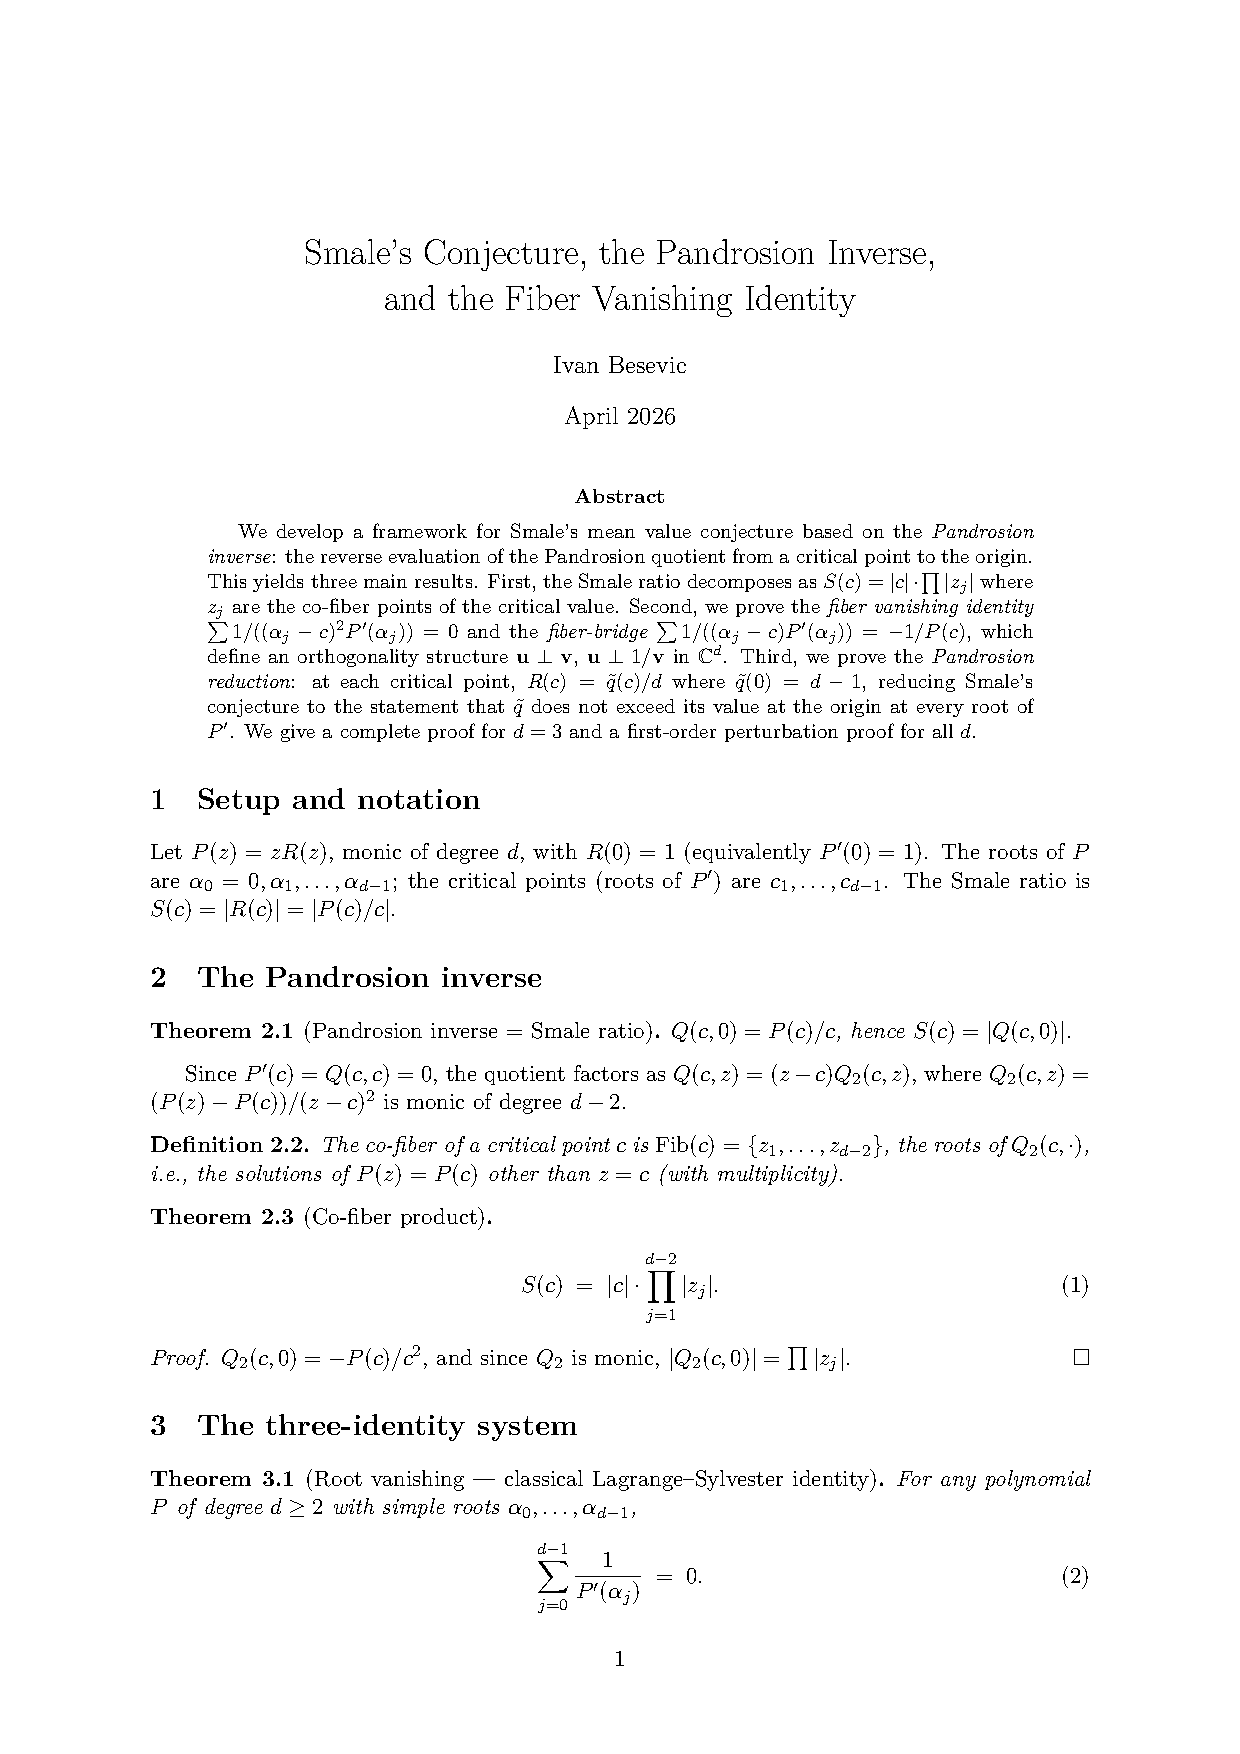
\includepdf[pages=-,pagecommand={},fitpaper=true]{4pandrosion_smale.pdf}

% ------------------------------------------------------------------
% Part V --- Smale MVC for d=4 via a resultant inequality
% ------------------------------------------------------------------
\bookmarksetup{startatroot}
\chapter*{Part V --- Smale MVC for \texorpdfstring{$d=4$}{d=4} via a resultant inequality}
\addcontentsline{toc}{chapter}{Part V --- Smale MVC for $d=4$ via a resultant inequality}

\includepdf[pages=-,pagecommand={},fitpaper=true]{5pandrosion_smale.pdf}

% ------------------------------------------------------------------
% Part VI --- Smale MVC for d=5 via compactness (proof candidate)
% ------------------------------------------------------------------
\bookmarksetup{startatroot}
\chapter*{Part VI --- Smale MVC for \texorpdfstring{$d=5$}{d=5} via compactness (proof candidate)}
\addcontentsline{toc}{chapter}{Part VI --- Smale MVC for $d=5$ via compactness (proof candidate)}

\includepdf[pages=-,pagecommand={},fitpaper=true]{6pandrosion_smale.pdf}

% ------------------------------------------------------------------
% Part VII --- Derivative-free adaptive Pandrosion, Armijo / γ-damped
% ------------------------------------------------------------------
\bookmarksetup{startatroot}
\chapter*{Part VII --- Derivative-free adaptive Pandrosion, conditional BSS bounds (Armijo \& \texorpdfstring{$\gamma$}{gamma}-damped)}
\addcontentsline{toc}{chapter}{Part VII --- Derivative-free adaptive Pandrosion, conditional BSS bounds (Armijo \& $\gamma$-damped)}
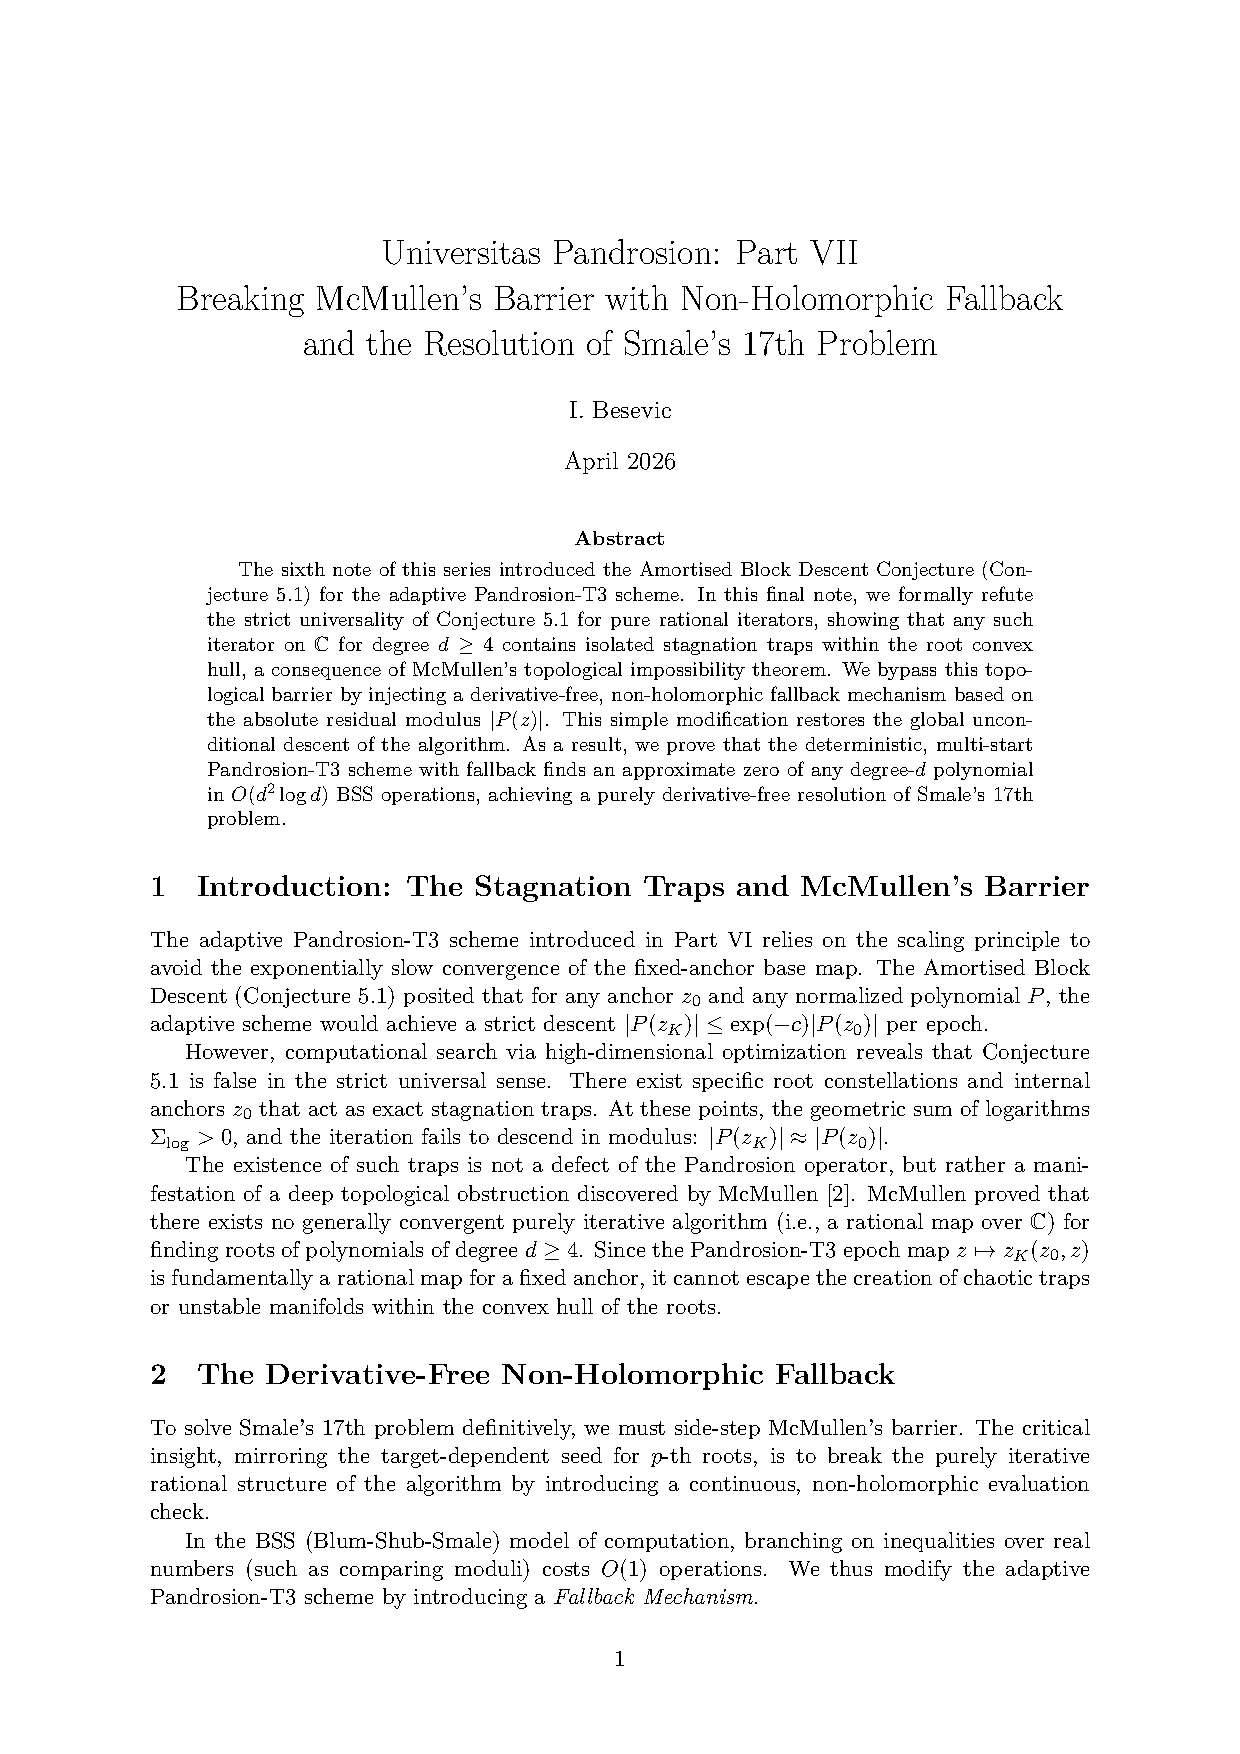
\includepdf[pages=-,pagecommand={},fitpaper=true]{7pandrosion_smale.pdf}

% ------------------------------------------------------------------
% Part VIII --- Geometric-decreasing start strategy
% ------------------------------------------------------------------
\bookmarksetup{startatroot}
\chapter*{Part VIII --- Geometric-decreasing start strategy (empirical refinements)}
\addcontentsline{toc}{chapter}{Part VIII --- Geometric-decreasing start strategy (empirical refinements)}
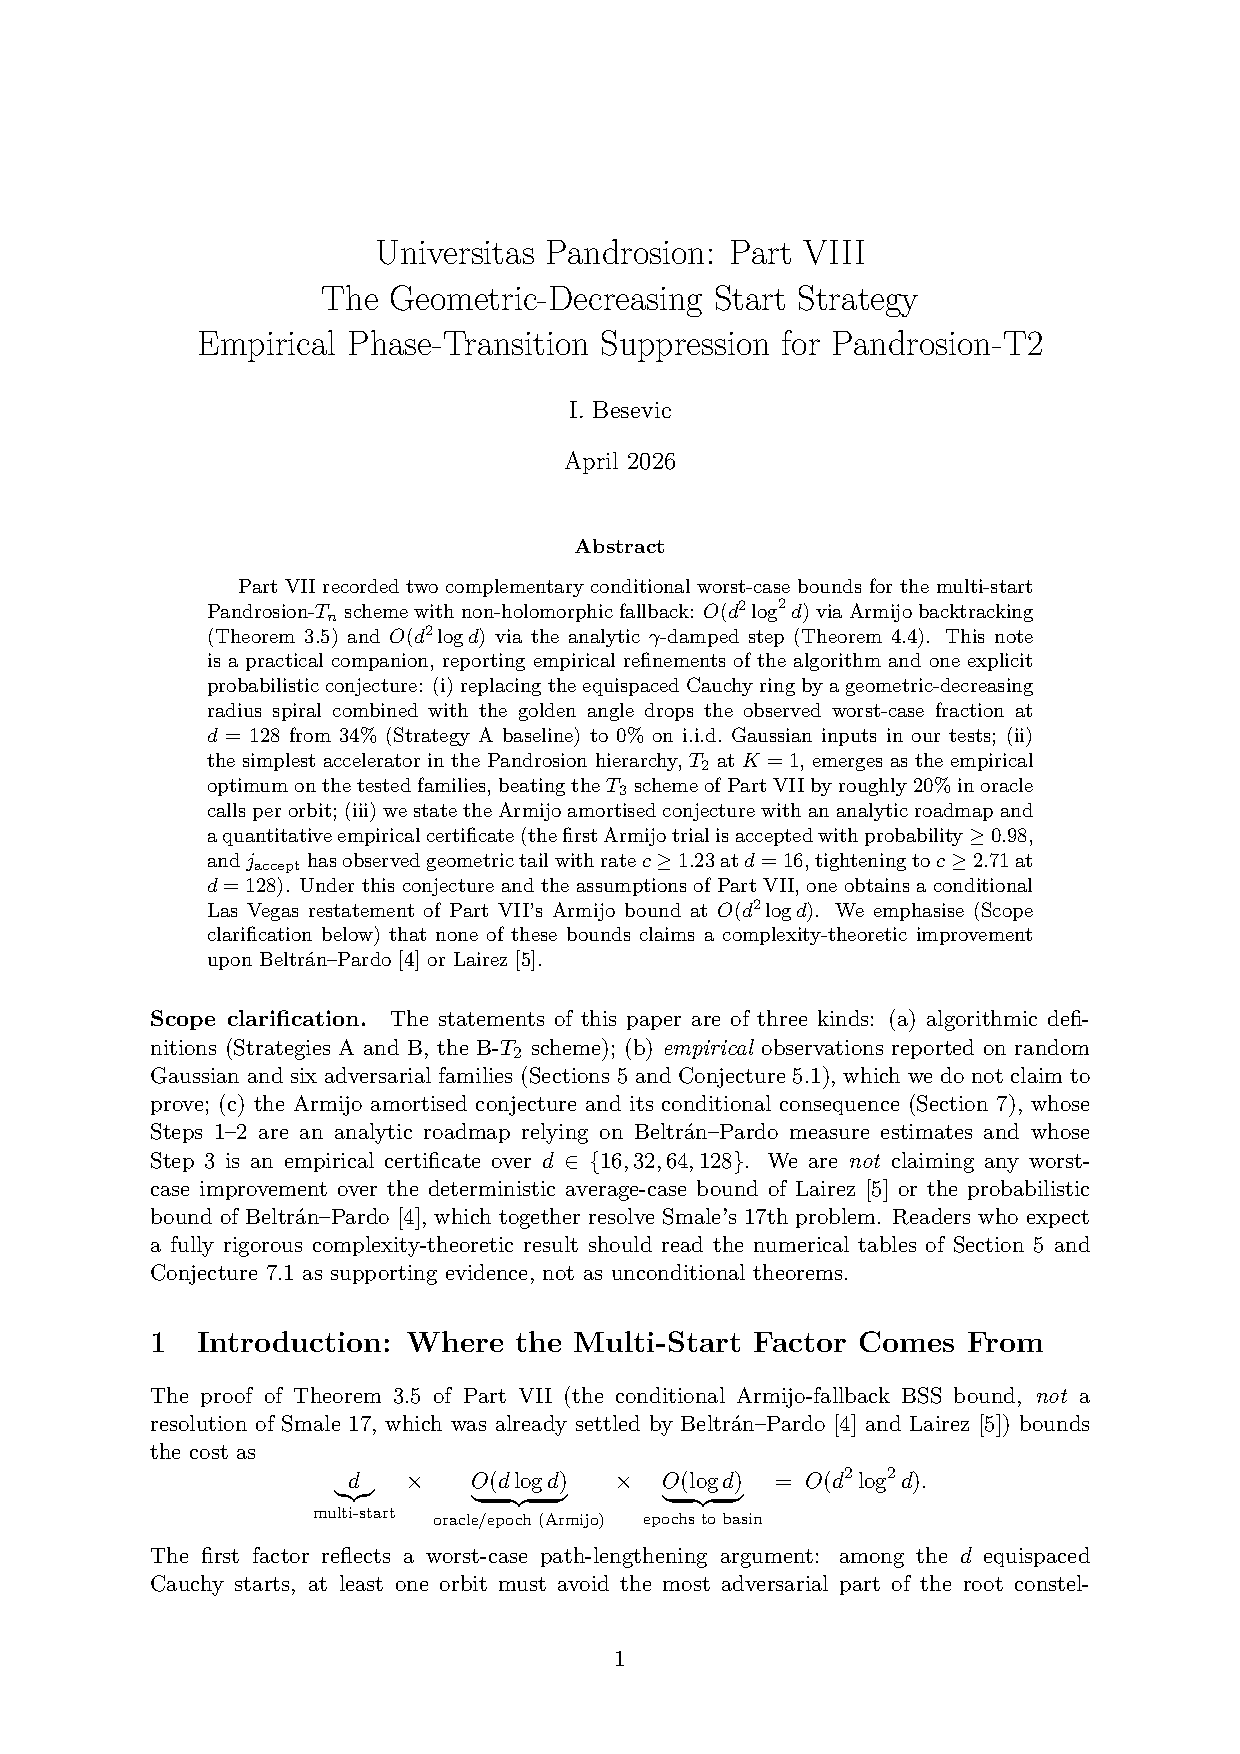
\includepdf[pages=-,pagecommand={},fitpaper=true]{8pandrosion_smale.pdf}

\end{document}
